The regular training procedure for a 4-feature model has a significant limitation. The model does not take into account the Feed-Forward application of the prediction output.
If the trained model has excellent input values, the output is expected to be within~1 \% miss accuracy.
\begin{figure*}[htbp]
    \centering
    % DST based tests
    \begin{subfigure}[b]{\columnwidth}
        \centering
        % \includesvg[width=\linewidth]{III_Conclussion/im_compare/FUDS-val-48.svg}
        \includesvg[width=\linewidth]{III_Conclussion/Models/Sadykov2020/FUDS-models/SMFUDS-val-9.svg}
        \caption{Regular training process snapshot}
        \label{subfig:regular_tr}
    \end{subfigure}
    \hfill
    \begin{subfigure}[b]{\columnwidth}
        \centering
        \includesvg[width=\linewidth]{III_Conclussion/Models/Sadykov2020/FUDS-models/SMFUDS-FF-9.svg}
        \caption{Feed-Forward validation process snapshot}
        \label{subfig:regular_ts}
    \end{subfigure}
    \caption{Comparison between training and testing accuracies of a 4-featured based model with a default training and testing loop}
    \label{fig:regular_tr}
\end{figure*}
% \begin{figure}[ht]%[htbp]
%     \centering
%     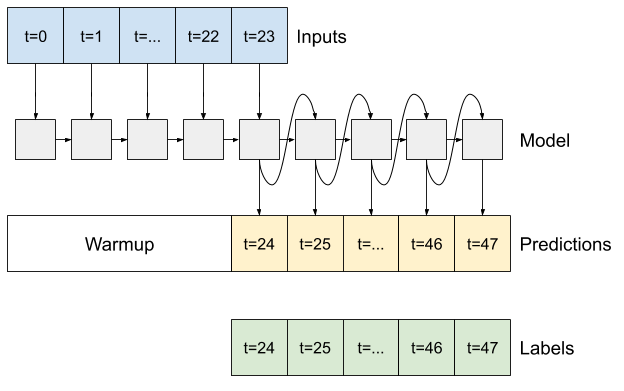
\includegraphics[width=0.7\linewidth]{II_Body/images/multistep_autoregressive.png}
%     \caption{documented way}
%     \label{fig:autoregressive}
% \end{figure}

%
%
Two subplots, \mbox{Figure~\ref{fig:regular_tr}}, demonstrate the prediction results of a four feature-based trained model against a single battery cycle of DST driving.
\mbox{Subfigure~\ref{subfig:regular_tr}} demonstrates the prediction based on the always known perfect State of Charge, opposite on \mbox{subfigure~\ref{subfig:regular_ts}} with only perfect initial, and every following sample gets fed-forward.
The loss axis has been dropped from plotting due to high inaccuracy.
\ifthenelse{\boolean{thesis}}{
    The implementation of this prediction method is presented in \mbox{Appendix~\ref{app:Feed-Forward}}.
}{}
It demonstrates how the appended charge output model accumulates the error with every dependant input in a single prediction.
If that output will be used for further prediction and the model keeps preserving the dependency, the miss accuracy value rises non-linearly.
The reason for that lies in the amount of weight the model places on the State of Charge input feature.
For a better weights balance, the training procedure must be modified to consider the possibility of an inaccuracy in the input charge data.
The diagram in \mbox{Figure~\ref{subfig:testing}} illustrates regular training and testing procedures for a model to produce output.
The implementation has been based on contributions from the original framework developers ~\cite{time_2020}.
Details have been attached to Appendix~\ref{app:AutoFeedback}.
\begin{figure*}[htbp]
    \centering
    % DST based tests
    \begin{subfigure}[b]{0.85\textwidth}
        \centering
        % 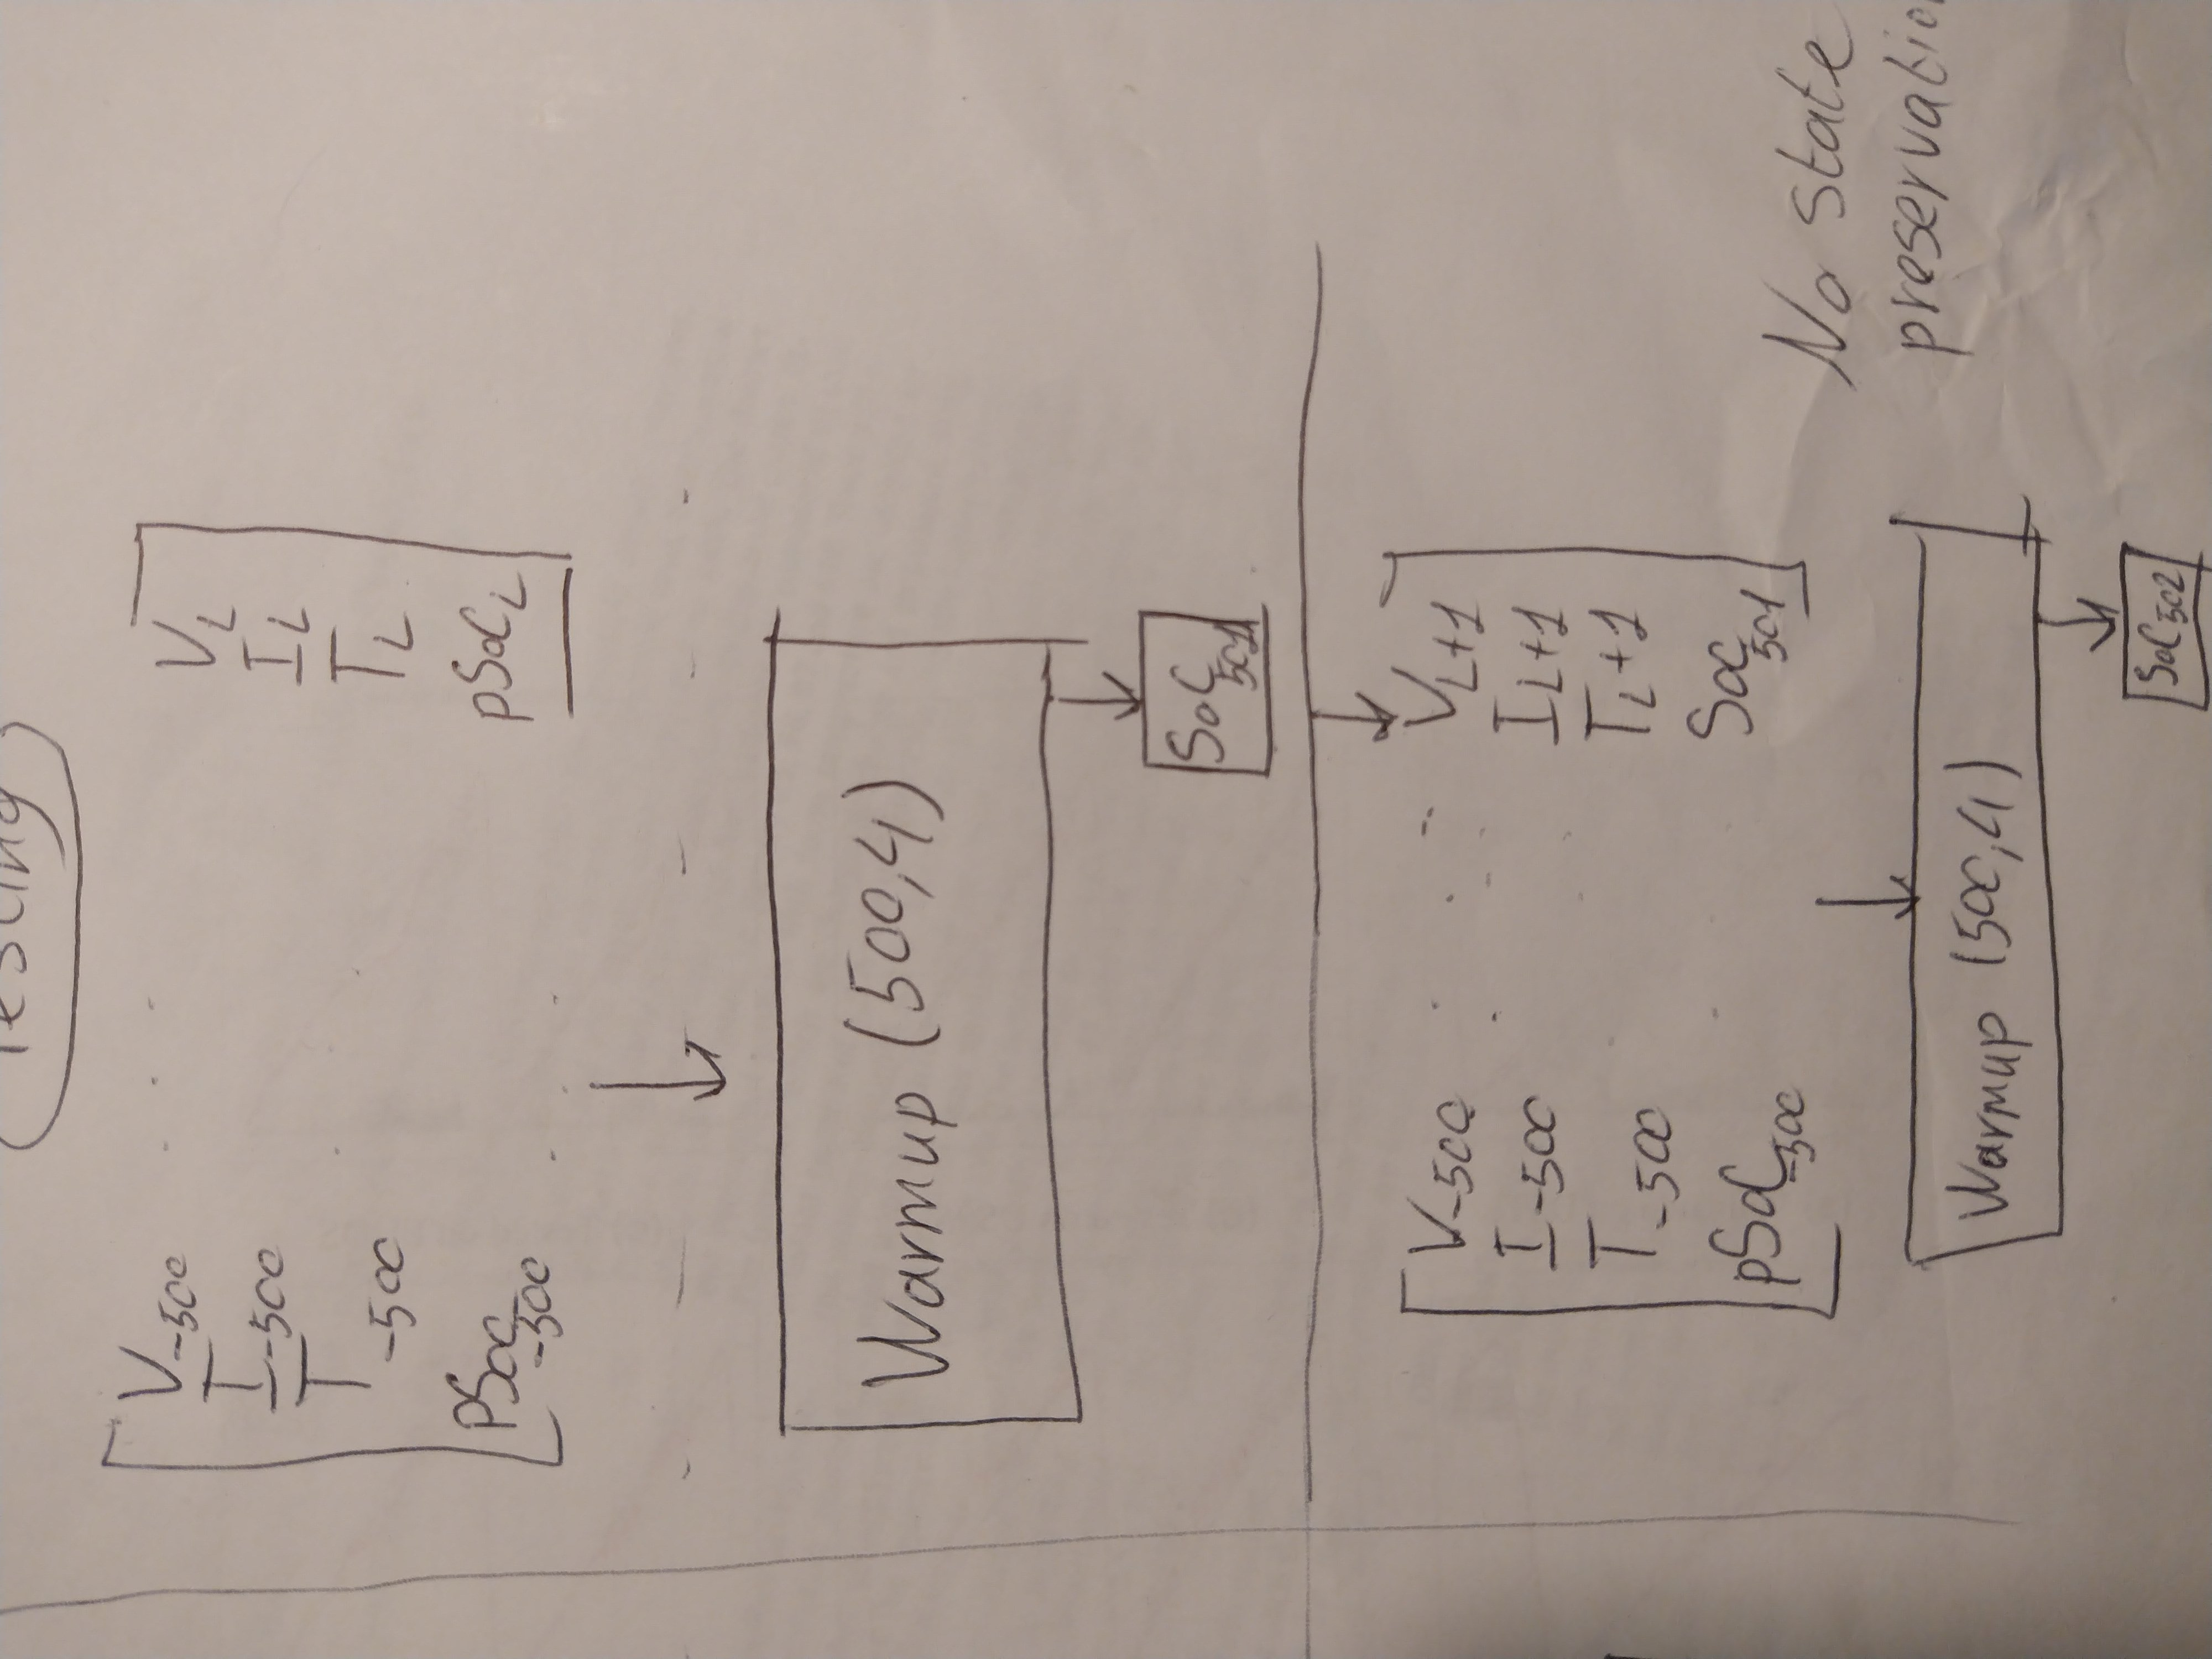
\includegraphics[width=\linewidth]{II_Body/images/IMG_20210524_133103.jpg}
        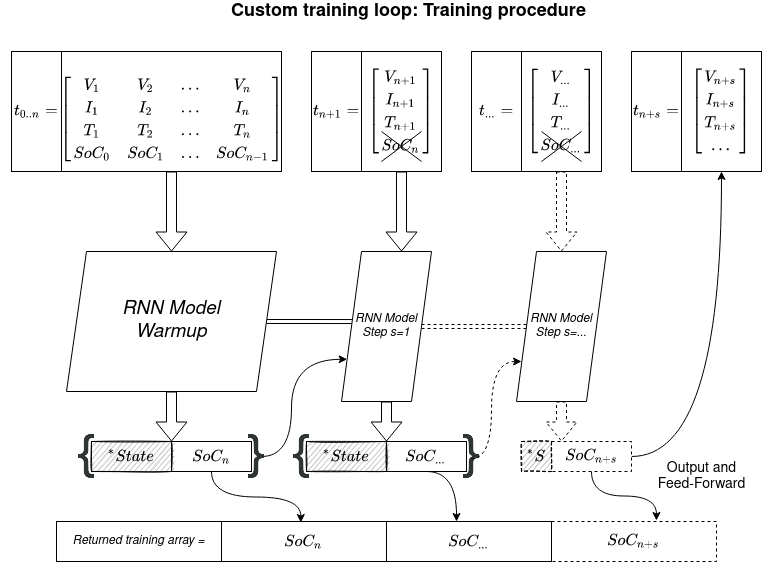
\includegraphics[width=\linewidth]{II_Body/images/Autoregression-Training.png}
        \caption{Custom autoregressive training procedure}
        \label{subfig:testing}
    \end{subfigure}
    \hfill
    \begin{subfigure}[b]{0.85\textwidth}
        \centering
        % 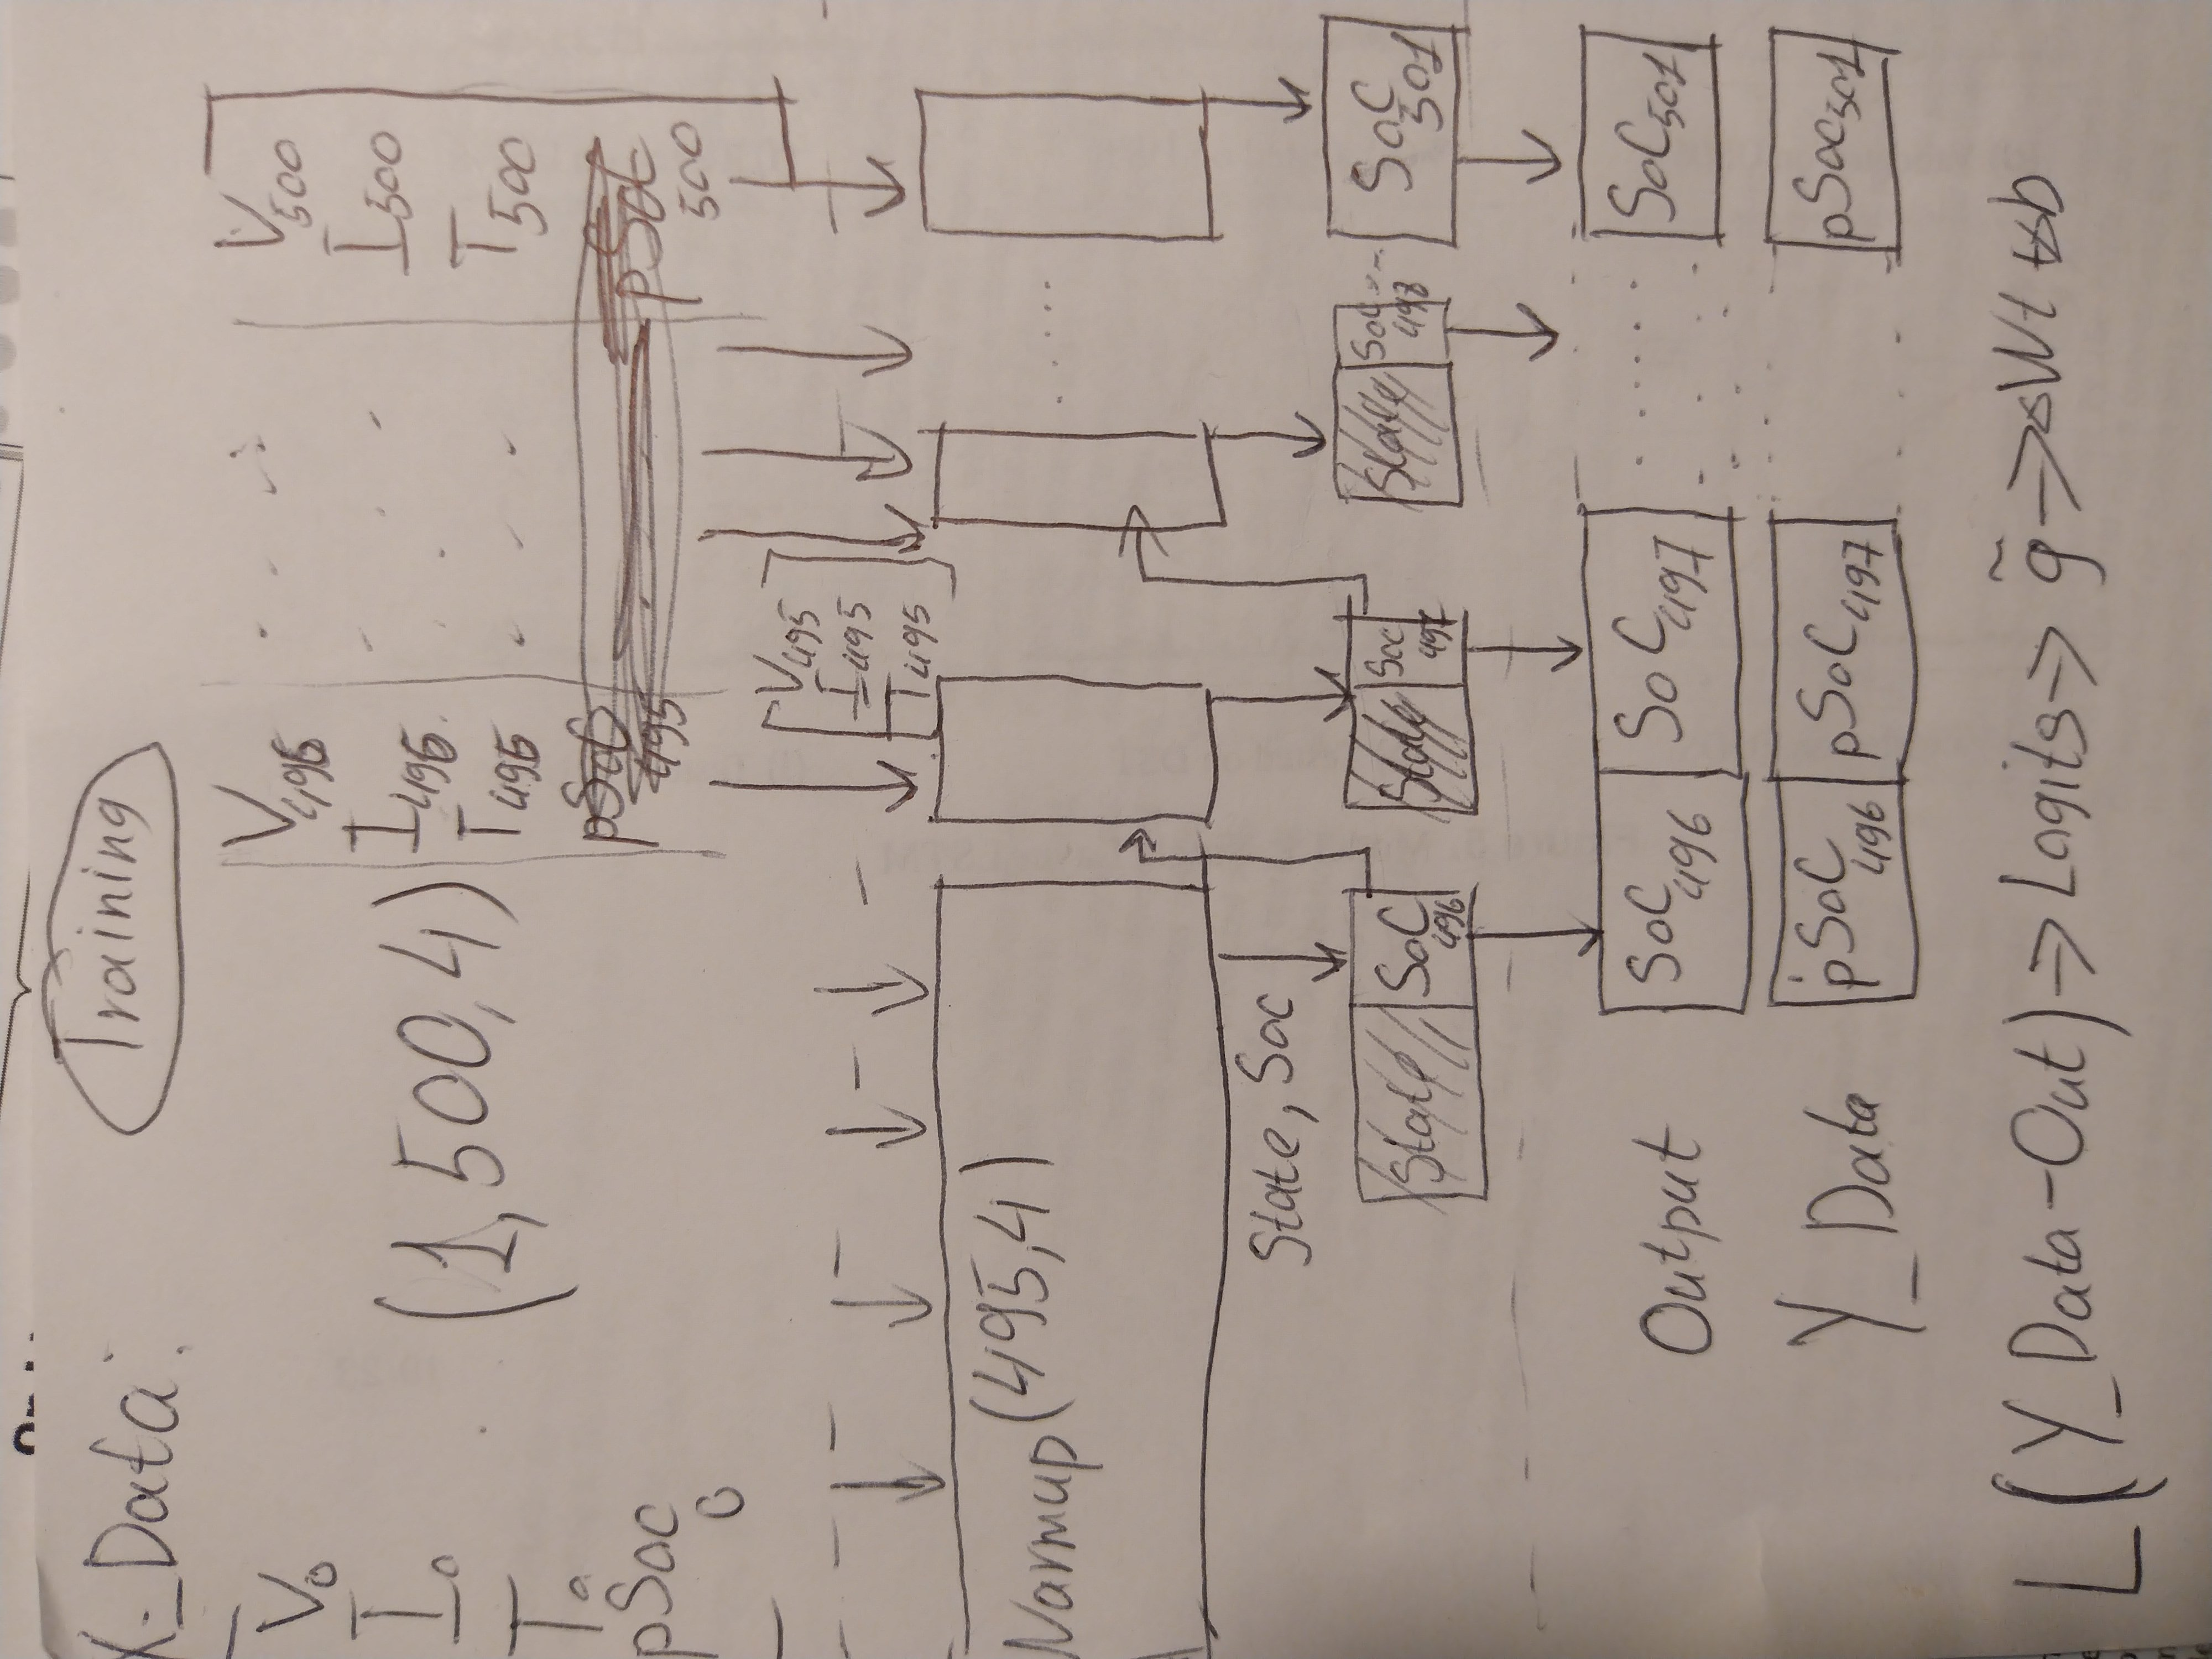
\includegraphics[width=\linewidth]{II_Body/images/IMG_20210524_133052.jpg}
        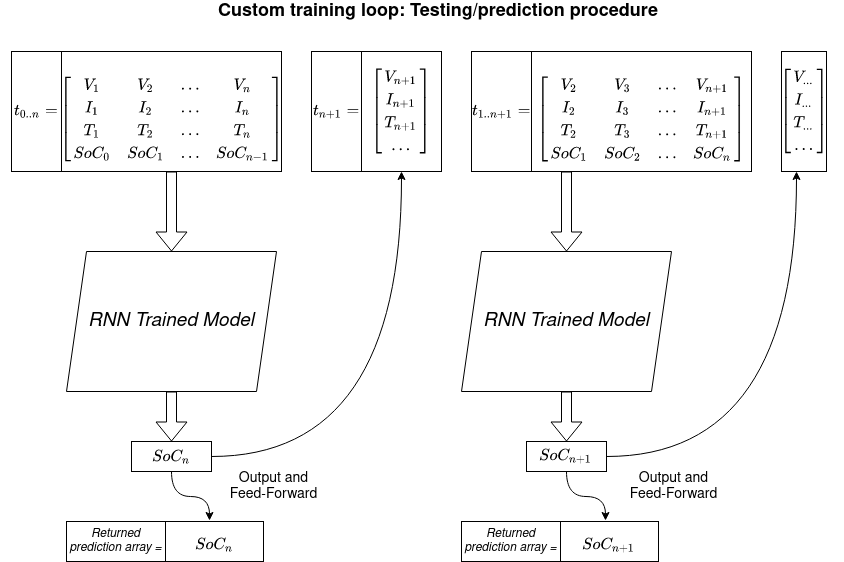
\includegraphics[width=\linewidth]{II_Body/images/Autoregression-Testing.png}
        \caption{Regular testing and validation procedure}
        \label{subfig:training}
    \end{subfigure}
    \caption{Comparison between training and testing accuracy of a 4-featured based model with a default training and testing loop.}
    \label{fig:training_testing}
\end{figure*}

%
%
The training procedure for the regular LSTM model must be modified to consider potential inaccuracy using the autoregression technique.
%\textcolor{red}{I do not feel comfortable referencing the documentation, but what choice do I have now.}
The diagram in \mbox{Subfigure~\ref{subfig:training}} demonstrates the procedure for the model call using autoregression.
Unlike regular LSTM, training and testing differentiate from each other.
If the testing procedure remained unchanged, the training performs multiple calls during a single-window sample processing.
Every new call outputs the results and feeds again into the same model, with one sample from each sensor.
Each output also contained a model state, containing the values stored in the cell, preserving dependency between model calls.
State output is used only for internal model processing.
Every output of every step has been stored as an array.
With a new approach, an optimiser will compare an array of predicted samples against the true values of the SoC.
This way meant to increase the model fit process.
The more output samples model returns during the training, the better the real-time prediction against aggressive driving profiles.
\mbox{Figure~\ref{fig:modefied_tr}} contains a similar test as without autoregression.
Even though the accuracy with tabled samples has decreased, its feed-forward prediction accuracy has significantly increased.
\begin{figure*}[htbp]
    \centering
    \begin{subfigure}[b]{\columnwidth}
        \centering
        \includesvg[width=\linewidth]{III_Conclussion/Models/Sadykov2021-30steps/FUDS-models/SMRFUDSval-19.svg}
        \caption{Modified training process}
    \end{subfigure}
    \begin{subfigure}[b]{\columnwidth}
        \centering
        \includesvg[width=\linewidth]{III_Conclussion/Models/Sadykov2021-30steps/FUDS-models/SMRFUDS-FF-19.svg}
        \caption{Feed-Forward validation process}
    \end{subfigure}
    \caption{Comparison between training and testing accuracies of a 4-featured based model with a modified training and default testing loop}
    \label{fig:modefied_tr}
\end{figure*}